\documentclass[twocolumn]{revtex4}

\usepackage{graphicx}
\usepackage{amsmath}

\begin{document}

\section{Introduction}

\section{Computational method}

Argon atoms were placed in a crystal structure at a given temperature, then evolved in time while logging a number of properties of the system as a function of time, including:
\begin{itemize}
\item Temperature
\item Total energy
\item Position
\item Velocity
\end{itemize}

\subsection{Initialization}

\subsubsection{Crystal structure}

The atoms were placed in a face-cented cubic (FCC) configuration, where each ``unit cell'' consisted of 4 atoms positioned as illustrated in figure~\ref{fig:fcc}.

A collection of argon atoms in an $L \times L \times L$ box with $d$ FCC unit cells in each direction thus has a number density of $n = 4d^3/L^3$.

\begin{figure}[htb]
\begin{center}
\leavevmode
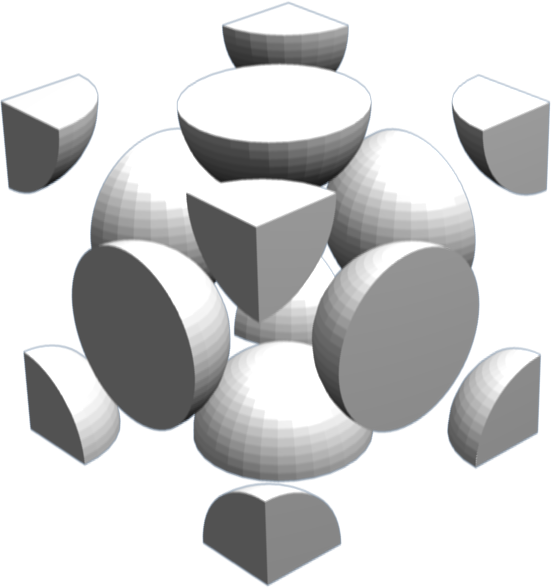
\includegraphics[width=0.45\textwidth]{fcc.png}
\end{center}
\caption{Face-centered cubic (FCC) lattice unit cell}
\label{fig:fcc}
\end{figure}

\subsubsection{Velocity distribution}

The velocity of each argon atom was set according to a Maxwell-Boltzmann distribution---i.e., a Gaussian distribution for each axis of the velocity. I used the Box-Muller algorithm to generate Gaussian-distributed numbers:

\begin{align}
z_1 &= \sqrt{-2 \ln u_1} \cos{2 \pi u_2}\\
z_2 &= \sqrt{-2 \ln u_1} \sin{2 \pi u_2},
\end{align}

where $u_1, u_2$ are uniformly distributed random numbers on $(0,1]$ and $z_1, z_2$ are Gaussian distributed random numbers. This caused the argon atoms to have speeds distributed with a Maxwell-Boltzmann distribution as shown in figure~\ref{fig:vel-dist}.

\begin{figure}[htb]
\begin{center}
\leavevmode
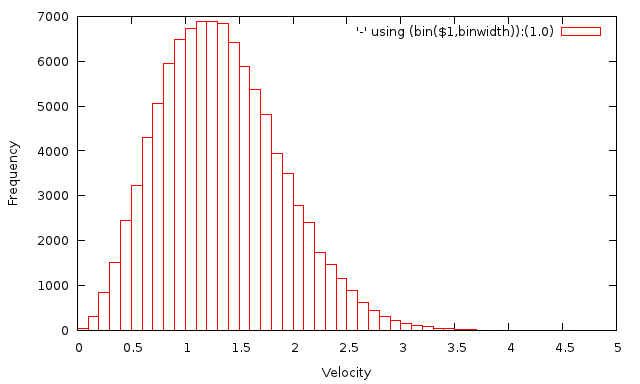
\includegraphics[width=0.45\textwidth]{vel-dist.png}
\end{center}
\caption{Maxwell-Boltzmann speed distribution of $10^4$ argon atoms}
\label{fig:vel-dist}
\end{figure}

The velocities of the atoms were then scaled up to the target temperature by scaling the velocities by a factor of $\sqrt{T_{\text{target}}/T}$.

\subsection{Simulation}

\subsubsection{Lennard-Jones potential}

The argon atoms are placed in a Lennard-Jones potential so that the potential of two atoms separated by a distance $r$ is

\begin{align}
V = 4\varepsilon \left( \left(\frac{\sigma}{r}\right)^{12} - \left(\frac{\sigma}{r}\right)^6 \right),
\end{align}

where $\sigma \approx 3.405\cdot10^{-10}$ m, $\varepsilon \approx 1.654\cdot10^{-21}$ J, and the mass $m \approx 6.69\cdot10^{-26}$ kg for argon. In the simulation, the units are normalized so that $\sigma = \varepsilon = m = 1$, so the potential is:

\begin{align}
V = 4 \left( \left(\frac{1}{r}\right)^{12} - \left(\frac{1}{r}\right)^6 \right).
\end{align}

The force on an atom is determined by the distances to all other atoms:

\begin{align}
\mathbf{f}_{i} = -24 \sum_{j\ne i} \left( \frac{2}{r_{ij}^{14}} - \frac{1}{r_{ij}^8} \right),
\end{align}

where $\mathbf{f}_i$ is the force on particle $i$ and $r_{ij}$ denotes the distance from particle $i$ to particle $j$.

\subsubsection{Verlet algorithm}

The simulation steps forward using the Verlet algorithm:

\begin{align}
X_{t+\delta t} &= X_t + V_t \delta t + F_t \frac{\delta t^2}{2}\\
F_{t+\delta t} &= \text{Lennard-Jones}(X_{t+\delta t})\\
V_{t+\delta t} &= V_t + (F_{t+\delta t} + F_t) \frac{\delta t}{2},
\end{align}

where $X$, $F$, and $V$ are matrices representing the positions, forces, and velocities of each argon atom. The subscript on each of these matrices denotes the simulation time the matrix represents the state of---for example, $X_{t+\delta t}$ represents the positions of the particles at $\delta t$ time units after the time $t$.

\subsubsection{Periodic boundaries}

In order to simulate a larger system, the simulation uses periodic boundary conditions; i.e., the atoms lie in a three-dimensional torus. However, this can cause the particles to attain a ``drift'', or non-zero center of mass velocity, due to numerical errors. To counteract this, the center of mass velocity of the system is zeroed before each timestep.

\subsection{Observable values}

\subsubsection{Kinetic energy}

To find the kinetic energy, the squared velocities of the atoms are summed up and divided by 2. Because $m=1$ (by definition), that term is removed.

\begin{align}
KE = \frac{1}{2} \sum_i m_i |\mathbf{v}_i|^2 = \frac{1}{2} \sum_i |\mathbf{v}_i|^2
\end{align}

\subsubsection{Temperature}

The temperature is calculated by the kinetic energy with

\begin{align}
\frac{3}{2} (N-1) k_B T &= \frac{1}{2} \sum_i |\mathbf{v}_i|^2 = KE\\
\implies & T = \frac{2}{3 k_B (N-1)} KE.
\end{align}

\subsubsection{Mean square distance}

In order to track the mean square distance of each atom from its original position, the simulation uses an extra variable $\mathbf{disp}$ that keeps track of a atom's displacement regardless of periodic boundary conditions. The mean square displacement is then defined as

\begin{align}
MSD = \frac{1}{N} \sum_i |\mathbf{disp}_i|^2 = \frac{1}{N} \sum_i |\mathbf{x}_t - \mathbf{x}_0|^2.
\end{align}

\section{Results}

\subsection{Test of two atoms in a Lennard-Jones potential}

In order to make sure the Lennard-Jones potential and Verlet algorithm were functioning correctly, I implemented a test case with two argon atoms separated by a distance of 2 length units in a Lennard-Jones potential. Figure~\ref{fig:lj-pos} shows the positions of the two argon atoms as a function of time---this shows the repulsive force of the potential at close ranges and the attractive force at farther ranges. Figure~\ref{fig:energy-cons} shows the total energy of the system as a function of time. Note that there is some instability when the atoms are close (strong forces lead to numerical errors), but the total energy returns to the correct value once the atoms are farther apart.

\begin{figure}[htb]
\begin{center}
\leavevmode
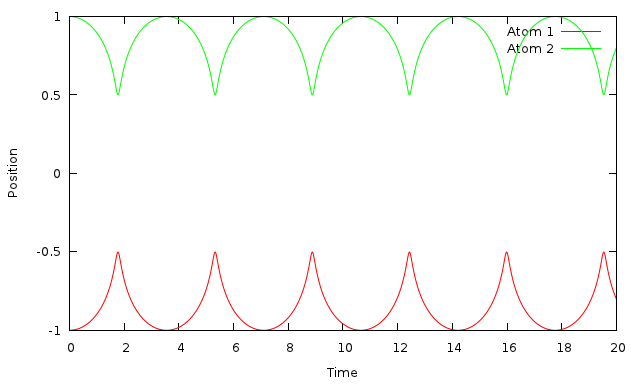
\includegraphics[width=0.45\textwidth]{lj-pos.png}
\end{center}
\caption{Position of two argon atoms in a Lennard-Jones potential}
\label{fig:lj-pos}
\end{figure}

\begin{figure}[htb]
\begin{center}
\leavevmode
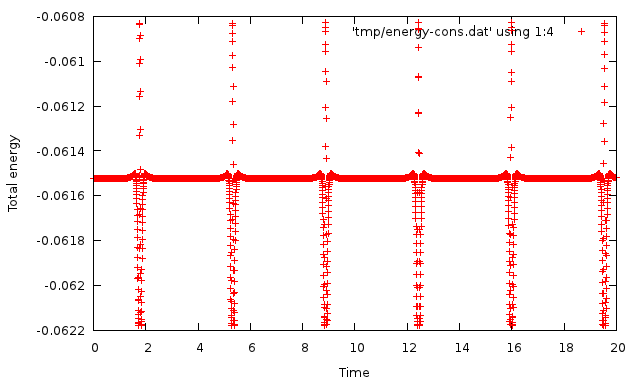
\includegraphics[width=0.45\textwidth]{energy-cons.png}
\end{center}
\caption{Total energy of a system with two argon atoms in a Lennard-Jones potential}
\label{fig:energy-cons}
\end{figure}

\subsection{Energy-temperature relation}

%E(T)=1/1.00098515425165*log(T/0.0219299261072685)
%T(E)=0.0219299261072685*exp(1.00098515425165*E)

\begin{figure}[htb]
\begin{center}
\leavevmode
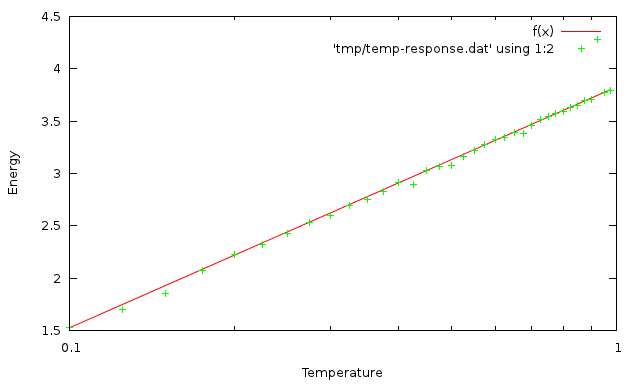
\includegraphics[width=0.45\textwidth]{temp-response.png}
\end{center}
\caption{Logarithmic relation of the temperature and total energy of a system. The logarithmic fit in the plot is defined by $E(T) = \ln(T/0.022)$.}
\label{fig:temp-response}
\end{figure}

\subsection{Mean square displacement}

\section{Conclusions}

\end{document}
